\documentclass[10pt,utf8,presentation,notheorems,xcolor=dvipsnames,compress]{beamer}
\usepackage{doclad}

%Тут можно вставить дополнительные пакеты

\title[Информационная система]{
Информационная система \newline «Better Row»
}

\author[Абдулов И.А.]{
  Абдулов Илья Александрович K3121
}

\date{23 декабря 2022}

\begin{document}

\begin{frame}
\titlepage
\end{frame}

\section<presentation>*{Содержание}

\begin{frame}
\frametitle{Содержание}
\tableofcontents
\end{frame}

\section{Введение}
\begin{frame}
\frametitle{Введение}
\begin{block}{Идея приложения «Better Row»}
Приложение «Better Row» найдет применение среди спортивных клубов и
удовлетворит потребности спортсменов в программном обеспечении для тренировок. Эта информационная система представляет из себя приложение, куда пользователь заносит данные своих тренировок, чтобы приложение показывало и сохраняло текущие показатели и прогресс. Использование приложения придаст
тренировкам осознанности, что поможет в достижении лучшего результата.
\end{block}

%\begin{block}{Цель курсовой работы}
%Целью данной работы является описание предметной области функционирования и основной идеи будущего мобильного приложения.
%\end{block}

\end{frame}

\section{Описание Better Row}

\subsection{Назначение и пользователи Better Row}
\begin{frame}
\frametitle{Назначение и пользователи Better Row}

\begin{block}{Назначение приложения}
Мобильное приложение позволит пользователю сохранять данные о
своих тренировках на гребном тренажере, чтобы в дальнейшем иметь возможность их просмотреть и проанализировать. Приложение поможет следить за показателями тренировок, видеть прогресс и иметь возможность поделиться результатами с тренером по сети Интернет.
\end{block}

\begin{block}{Основные пользователи}
Основными пользователями системы будут являться любители академической гребли и участники студенческой гребной лиги России.
\end{block}
\end{frame}

\subsection{Планируемый набор функций и прототип интерфейса}

\begin{frame}
\frametitle{Главное меню приложения}

\begin{columns}[c]

\begin{column}{.5\textwidth}
Планируется реализовать три вкладки в главном меню: результаты и статистика, расписание тренировок, настройки приложения.
\end{column}

\begin{column}{.5\textwidth}
\begin{center}
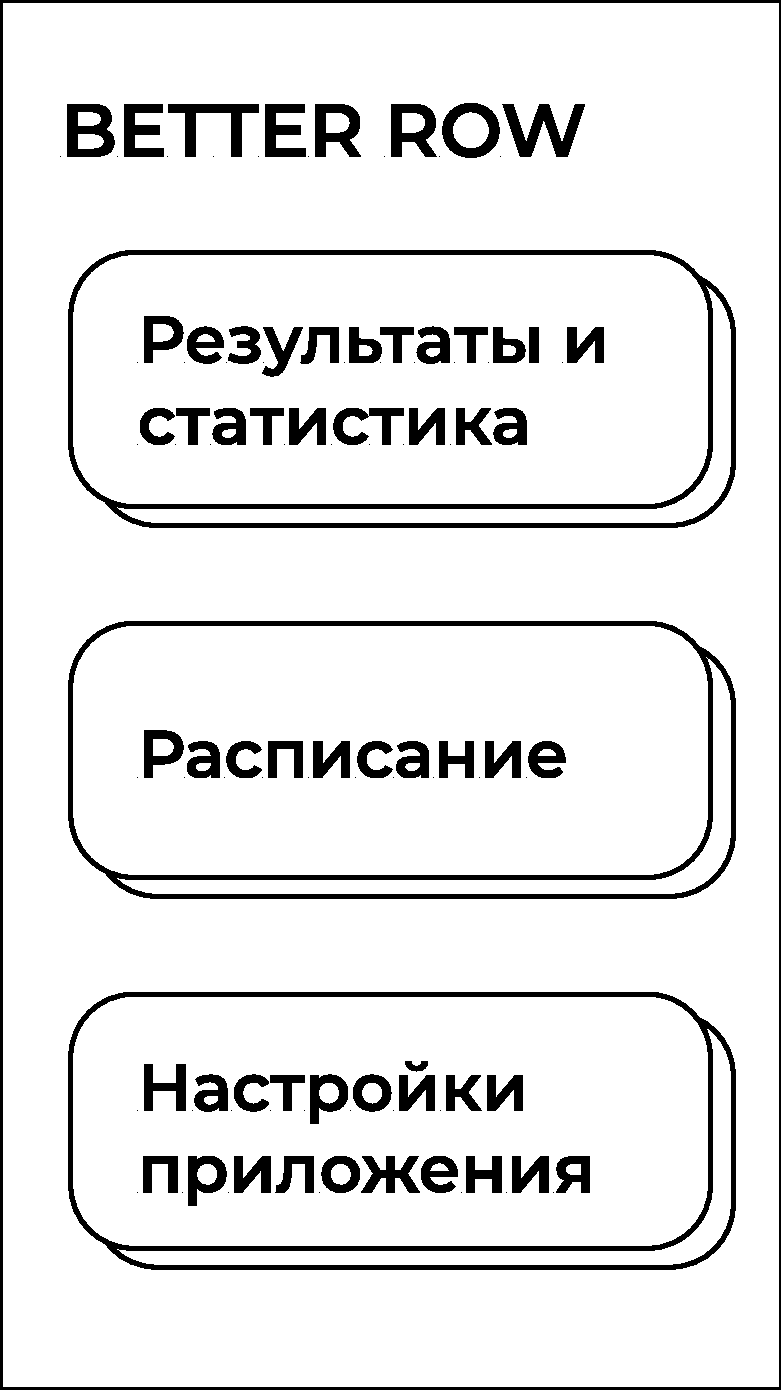
\includegraphics[scale=0.29]{iPhone 8 - 3.pdf}%
\end{center}
\end{column}

\end{columns}
\end{frame}

\begin{frame}
\frametitle{Pезультаты и статистика}

\begin{columns}[c]

\begin{column}{.5\textwidth}
Во вкладке результатов и статистики пользователь сможет перемещаться по дням и
либо просматривать результаты тренировки в этот день, либо добавлять
информацию о тренировке. При добавлении тренировки пользователь вводит дистанцию, время, темп заплыва на гребном тренажере – обязательные
показатели, а также пульс после заплыва – опциональную характеристику
для ввода. 
\end{column}

\begin{column}{.5\textwidth}
\begin{center}
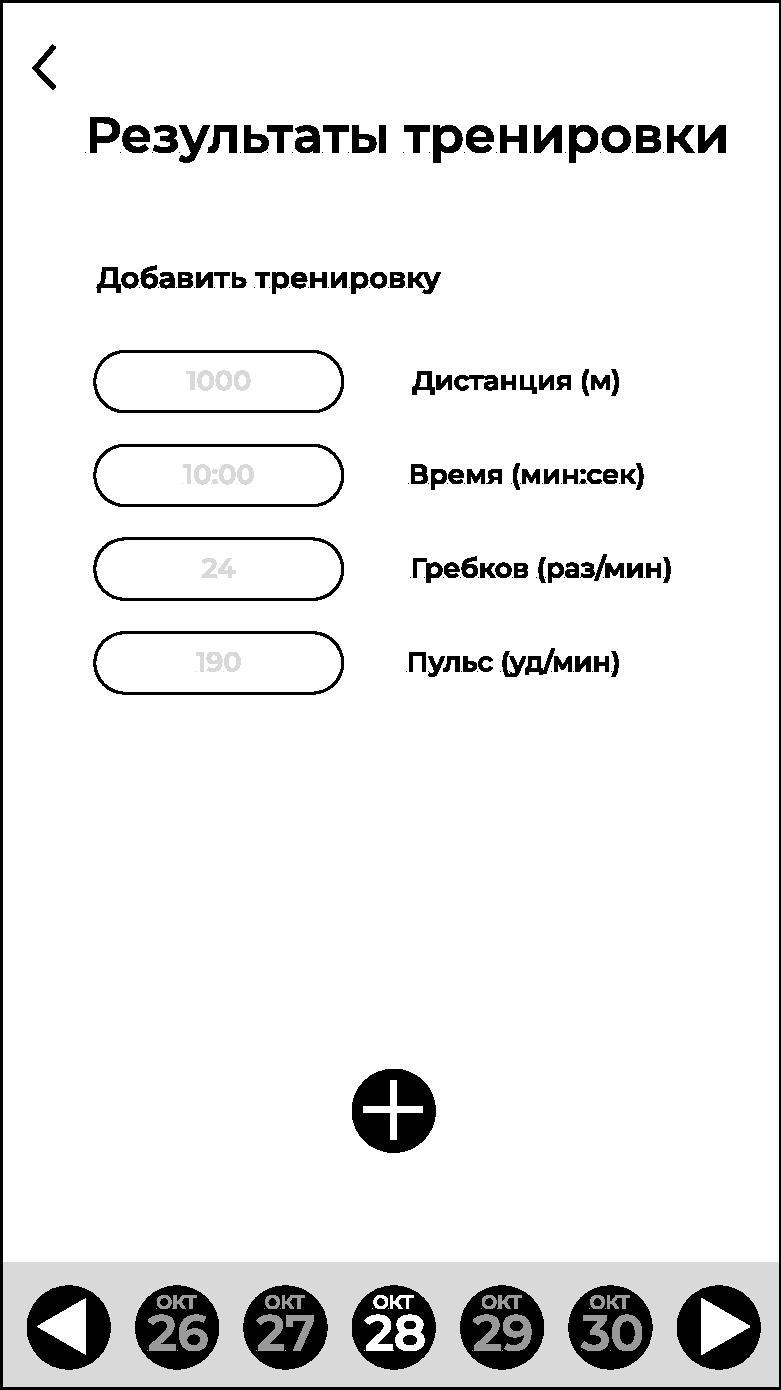
\includegraphics[scale=0.29]{iPhone 8 - 2}%
\end{center}
\end{column}

\end{columns}
\end{frame}

\begin{frame}
\frametitle{Pезультаты и статистика}
\begin{columns}[c]

\begin{column}{.5\textwidth}
При просмотре тренировок, которые уже были добавлены, к введённым показателям автоматически добавляется автоматически рассчитанная приложением
средняя скорость заплыва. Кроме того, реализованы функции просмотра изменения результата по сравнению с прошлыми тренировками.
\end{column}

\begin{column}{.5\textwidth}
\begin{center}
\includegraphics[scale=0.29]{iPhone 8 - 1}%
\end{center}
\end{column}

\end{columns}
\end{frame}

\begin{frame}
\frametitle{Расписание тренировок}
\begin{columns}[c]

\begin{column}{.5\textwidth}
Во вкладке расписания тренировок будут указанные дни недели, в которые проходят тренировки, время и место занятий секции. Если расписание
тренировок поменяется, то, используя функцию, его можно будет изменить
в той же вкладке.
\end{column}

\begin{column}{.5\textwidth}
\begin{center}
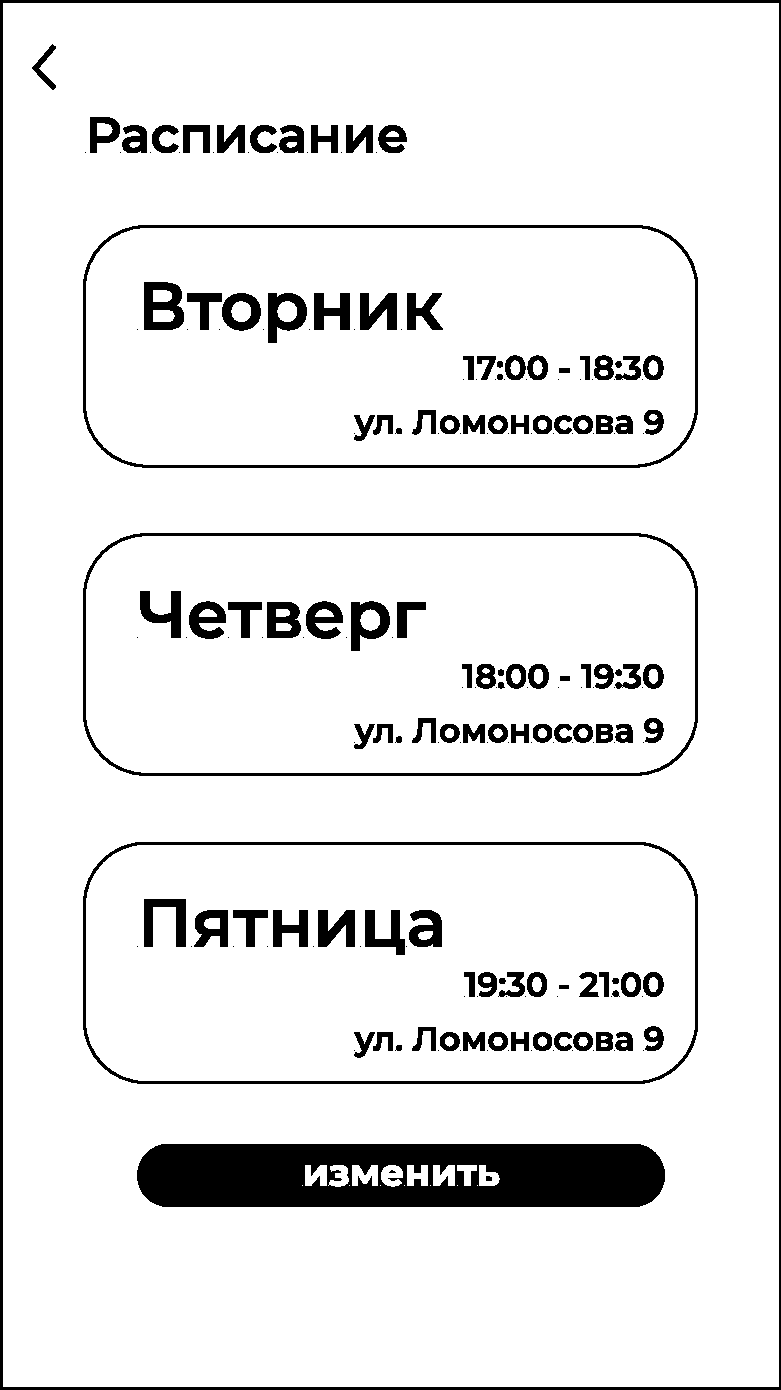
\includegraphics[scale=0.29]{iPhone 8 - 4}%
\end{center}
\end{column}

\end{columns}
\end{frame}


\section{Аналоги}
\begin{frame}
\frametitle{Watersports Tracker}
Аналогичное разрабатываемой системе приложение, которое предоставляет статистику о тренировке на воде, отслеживая геолокацию смартфона.
\begin{center}
\includegraphics[scale=0.3]{Watersports Tracker}%
\end{center}
\end{frame}

\begin{frame}
\frametitle{RowingCoach 4.0}
Аналогичное разрабатываемой системе приложение, которое предоставляет статистику и все показатели тренировки, отслеживая местоположение пользователя.
\begin{center}
\includegraphics[scale=0.3]{RowingCoach}%
\end{center}
\end{frame}

\section{Модели и диаграммы системы}

\subsection{Модель прецедентов и диаграмма активности}

\begin{frame}
\frametitle{Диаграмма вариантов использования системы}
\begin{center}
\includegraphics[scale=0.35]{UseCaseDiagram.pdf}%
\end{center}
\end{frame}

\begin{frame}
\frametitle{Диаграмма активности для ключевого прецедента}
\begin{center}
\includegraphics[scale=0.35]{ActivityDiagram.pdf}%
\end{center}
\end{frame}

\subsection{Методология IDEF0}

\begin{frame}
\frametitle{Функциональная модель в стандарте IDEF0}
\begin{center}
\includegraphics[scale=0.18]{01_A0.jpg}%
\end{center}
\end{frame}

\begin{frame}
\frametitle{Первый уровень декомпозиции "Аналитика тренировки спортсмена"}
\begin{center}
\includegraphics[scale=0.18]{02_A0.jpg}%
\end{center}
\end{frame}

\begin{frame}
\frametitle{Второй уровень декомпозиции "Показ результатов тренировки и аналитика"}
\begin{center}
\includegraphics[scale=0.18]{03_A3.jpg}%
\end{center}
\end{frame}

\begin{frame}
\frametitle{Третий уровень декомпозиции "Вычисление средней скорости и прогресса алгоритмом"}
\begin{center}
\includegraphics[scale=0.18]{04_A32.jpg}%
\end{center}
\end{frame}

\subsection{Диаграммы DFD}

\begin{frame}
\frametitle{Контекстная диаграмма в стандарте DFD}
\begin{center}
\includegraphics[scale=0.35]{A-0_DFD_diagram.pdf}%
\end{center}
\end{frame}

\begin{frame}
\frametitle{Декомпозиция блока в стандарте DFD}
\begin{center}
\includegraphics[scale=0.35]{A0_DFD_diagram.pdf}%
\end{center}
\end{frame}

\section{Заключение}
\begin{frame}
\frametitle{Заключение}

\begin{block}{Цель курсовой работы была достигнута.}
Техническое задание на разработку информационной системы «Better
Row» составлено.
\end{block}

\begin{block}{Были решены следующие задачи:}
\begin{itemize}
 \item Описана основная идея мобильного приложения «Better Row»;
 \item Описано назначение и пользователи будущей ИС;
 \item Продемонстрирован интерфейс будущего мобильного приложения;
 \item Проанализирован рынок приложений на наличие аналогов системы;
 \item Представлены модели и диаграммы описываемой системы.
\end{itemize}
\end{block}

\end{frame}
\end{document}
